\documentclass[a4paper]{book}
\usepackage{makeidx}
\usepackage{natbib}
\usepackage{graphicx}
\usepackage{multicol}
\usepackage{float}
\usepackage{listings}
\usepackage{color}
\usepackage{ifthen}
\usepackage[table]{xcolor}
\usepackage{textcomp}
\usepackage{alltt}
\usepackage{ifpdf}
\ifpdf
\usepackage[pdftex,
            pagebackref=true,
            colorlinks=true,
            linkcolor=blue,
            unicode
           ]{hyperref}
\else
\usepackage[ps2pdf,
            pagebackref=true,
            colorlinks=true,
            linkcolor=blue,
            unicode
           ]{hyperref}
\usepackage{pspicture}
\fi
\usepackage[utf8]{inputenc}
\usepackage{mathptmx}
\usepackage[scaled=.90]{helvet}
\usepackage{courier}
\usepackage{sectsty}
\usepackage[titles]{tocloft}
\usepackage{doxygen}
\lstset{language=C++,inputencoding=utf8,basicstyle=\footnotesize,breaklines=true,breakatwhitespace=true,tabsize=8,numbers=left }
\makeindex
\setcounter{tocdepth}{3}
\renewcommand{\footrulewidth}{0.4pt}
\renewcommand{\familydefault}{\sfdefault}
\hfuzz=15pt
\setlength{\emergencystretch}{15pt}
\hbadness=750
\tolerance=750
\begin{document}
\hypersetup{pageanchor=false,citecolor=blue}
\begin{titlepage}
\vspace*{7cm}
\begin{center}
{\Large \-P\-A09\-\_\-\-Lab11\-\_\-\-Huffman\-\_\-\-Henry }\\
\vspace*{1cm}
{\large \-Generated by Doxygen 1.7.6.1}\\
\vspace*{0.5cm}
{\small Tue Nov 4 2014 23:54:33}\\
\end{center}
\end{titlepage}
\clearemptydoublepage
\pagenumbering{roman}
\tableofcontents
\clearemptydoublepage
\pagenumbering{arabic}
\hypersetup{pageanchor=true,citecolor=blue}
\chapter{\-Class \-Index}
\section{\-Class \-Hierarchy}
\-This inheritance list is sorted roughly, but not completely, alphabetically\-:\begin{DoxyCompactList}
\item \contentsline{section}{\-Queue$<$ \-Data\-Type $>$}{\pageref{class_queue}}{}
\begin{DoxyCompactList}
\item \contentsline{section}{\-Queue\-Array$<$ \-Data\-Type $>$}{\pageref{class_queue_array}}{}
\item \contentsline{section}{\-Queue\-Linked$<$ \-Data\-Type $>$}{\pageref{class_queue_linked}}{}
\end{DoxyCompactList}
\end{DoxyCompactList}

\chapter{\-Class \-Index}
\section{\-Class \-List}
\-Here are the classes, structs, unions and interfaces with brief descriptions\-:\begin{DoxyCompactList}
\item\contentsline{section}{\hyperlink{struct_account}{\-Account} }{\pageref{struct_account}}{}
\item\contentsline{section}{\hyperlink{struct_account_record}{\-Account\-Record} }{\pageref{struct_account_record}}{}
\item\contentsline{section}{\hyperlink{class_b_s_tree}{\-B\-S\-Tree$<$ Data\-Type, Key\-Type $>$} }{\pageref{class_b_s_tree}}{}
\item\contentsline{section}{\hyperlink{class_b_s_tree_1_1_b_s_tree_node}{\-B\-S\-Tree$<$ Data\-Type, Key\-Type $>$\-::\-B\-S\-Tree\-Node} }{\pageref{class_b_s_tree_1_1_b_s_tree_node}}{}
\item\contentsline{section}{\hyperlink{class_hash_table}{\-Hash\-Table$<$ Data\-Type, Key\-Type $>$} }{\pageref{class_hash_table}}{}
\item\contentsline{section}{\hyperlink{struct_index_entry}{\-Index\-Entry} }{\pageref{struct_index_entry}}{}
\item\contentsline{section}{\hyperlink{class_test_data}{\-Test\-Data} }{\pageref{class_test_data}}{}
\item\contentsline{section}{\hyperlink{struct_user}{\-User} }{\pageref{struct_user}}{}
\end{DoxyCompactList}

\chapter{\-File \-Index}
\section{\-File \-List}
\-Here is a list of all files with brief descriptions\-:\begin{DoxyCompactList}
\item\contentsline{section}{\hyperlink{config_8h}{config.\-h} }{\pageref{config_8h}}{}
\item\contentsline{section}{\hyperlink{_heap_8cpp}{\-Heap.\-cpp} \\*\-This program contains the basic function for manipulating data in the heap }{\pageref{_heap_8cpp}}{}
\item\contentsline{section}{\hyperlink{_heap_8h}{\-Heap.\-h} }{\pageref{_heap_8h}}{}
\item\contentsline{section}{\hyperlink{heapsort_8cs}{heapsort.\-cs} }{\pageref{heapsort_8cs}}{}
\item\contentsline{section}{\hyperlink{ossim_8cpp}{ossim.\-cpp} \\*\-This program uses a priority queue to simulate a line }{\pageref{ossim_8cpp}}{}
\item\contentsline{section}{\hyperlink{ossim_8cs}{ossim.\-cs} }{\pageref{ossim_8cs}}{}
\item\contentsline{section}{\hyperlink{_priority_queue_8cpp}{\-Priority\-Queue.\-cpp} \\*\-The priority queue uses the predefined heap functions to perform basic priority queue operations }{\pageref{_priority_queue_8cpp}}{}
\item\contentsline{section}{\hyperlink{_priority_queue_8h}{\-Priority\-Queue.\-h} }{\pageref{_priority_queue_8h}}{}
\item\contentsline{section}{\hyperlink{show11_8cpp}{show11.\-cpp} }{\pageref{show11_8cpp}}{}
\item\contentsline{section}{\hyperlink{test11_8cpp}{test11.\-cpp} }{\pageref{test11_8cpp}}{}
\item\contentsline{section}{\hyperlink{test11hs_8cpp}{test11hs.\-cpp} }{\pageref{test11hs_8cpp}}{}
\item\contentsline{section}{\hyperlink{test11pq_8cpp}{test11pq.\-cpp} }{\pageref{test11pq_8cpp}}{}
\end{DoxyCompactList}

\chapter{\-Class \-Documentation}
\hypertarget{class_greater}{\section{\-Greater$<$ \-Key\-Type $>$ \-Class \-Template \-Reference}
\label{class_greater}\index{\-Greater$<$ Key\-Type $>$@{\-Greater$<$ Key\-Type $>$}}
}
\subsection*{\-Public \-Member \-Functions}
\begin{DoxyCompactItemize}
\item 
bool \hyperlink{class_greater_a79d9cb7121723ee9d65b11cb2fce0379}{operator()} (const \-Key\-Type \&a, const \-Key\-Type \&b) const 
\end{DoxyCompactItemize}
\subsubsection*{template$<$typename Key\-Type = int$>$ class Greater$<$ Key\-Type $>$}



\subsection{\-Member \-Function \-Documentation}
\hypertarget{class_greater_a79d9cb7121723ee9d65b11cb2fce0379}{\index{\-Greater@{\-Greater}!operator()@{operator()}}
\index{operator()@{operator()}!Greater@{\-Greater}}
\subsubsection[{operator()}]{\setlength{\rightskip}{0pt plus 5cm}template$<$typename Key\-Type  = int$>$ bool {\bf \-Greater}$<$ \-Key\-Type $>$\-::operator() (
\begin{DoxyParamCaption}
\item[{const \-Key\-Type \&}]{a, }
\item[{const \-Key\-Type \&}]{b}
\end{DoxyParamCaption}
) const\hspace{0.3cm}{\ttfamily  \mbox{[}inline\mbox{]}}}}\label{class_greater_a79d9cb7121723ee9d65b11cb2fce0379}


\-The documentation for this class was generated from the following file\-:\begin{DoxyCompactItemize}
\item 
\hyperlink{test11_8cpp}{test11.\-cpp}\end{DoxyCompactItemize}

\hypertarget{class_heap}{\section{\-Heap$<$ \-Data\-Type, \-Key\-Type, \-Comparator $>$ \-Class \-Template \-Reference}
\label{class_heap}\index{\-Heap$<$ Data\-Type, Key\-Type, Comparator $>$@{\-Heap$<$ Data\-Type, Key\-Type, Comparator $>$}}
}


{\ttfamily \#include $<$\-Heap.\-h$>$}

\subsection*{\-Public \-Member \-Functions}
\begin{DoxyCompactItemize}
\item 
\hyperlink{class_heap_ae17e34e3c86d88263a8fdf80b9ba78fc}{\-Heap} (int max\-Number=\hyperlink{class_heap_a967c19732a20a72e8e824402ad6763c8}{\-D\-E\-F\-A\-U\-L\-T\-\_\-\-M\-A\-X\-\_\-\-H\-E\-A\-P\-\_\-\-S\-I\-Z\-E})
\item 
\hyperlink{class_heap_a97e3b462be1c6af31d7519546bba8907}{\-Heap} (const \hyperlink{class_heap}{\-Heap} \&other)
\item 
\hyperlink{class_heap}{\-Heap} \& \hyperlink{class_heap_a5ed119341c39bcea1437321d4247dd40}{operator=} (const \hyperlink{class_heap}{\-Heap} \&other)
\item 
\hyperlink{class_heap_a555ade7891007de959bef0ee53e28767}{$\sim$\-Heap} ()
\item 
void \hyperlink{class_heap_aa68cf80454ab1b246fa723612805a91e}{insert} (const \-Data\-Type \&new\-Data\-Item)  throw ( logic\-\_\-error )
\item 
\-Data\-Type \hyperlink{class_heap_a4a18bfdacd897c45fc3da13f22b8930d}{remove} ()  throw ( logic\-\_\-error )
\item 
void \hyperlink{class_heap_a19a78c8eae2cf7c8253e34e54d86ed73}{clear} ()
\item 
bool \hyperlink{class_heap_ab8fa26d416ac0e27dfcbf18c54f8f73f}{is\-Empty} () const 
\item 
bool \hyperlink{class_heap_ac9111b884c74a376240e0155a788756e}{is\-Full} () const 
\item 
void \hyperlink{class_heap_a3ae1e1f27a145749c8b9f2da777cb8bc}{show\-Structure} () const 
\item 
void \hyperlink{class_heap_a4bdb1772ea92899de245d6cbd217d085}{write\-Levels} () const 
\end{DoxyCompactItemize}
\subsection*{\-Static \-Public \-Attributes}
\begin{DoxyCompactItemize}
\item 
static const int \hyperlink{class_heap_a967c19732a20a72e8e824402ad6763c8}{\-D\-E\-F\-A\-U\-L\-T\-\_\-\-M\-A\-X\-\_\-\-H\-E\-A\-P\-\_\-\-S\-I\-Z\-E} = 10
\end{DoxyCompactItemize}
\subsection*{\-Private \-Member \-Functions}
\begin{DoxyCompactItemize}
\item 
void \hyperlink{class_heap_a49a54dd4782e6c68f14a5df3ba4da7af}{show\-Subtree} (int index, int level) const 
\item 
int \hyperlink{class_heap_a16bf14bc857237c3d19f2583d8bdee0e}{get\-Left} (int index) const 
\item 
int \hyperlink{class_heap_ad748987560679176248ee980978e9a2f}{get\-Right} (int index) const 
\item 
int \hyperlink{class_heap_a0a67a2c91d1beefb12116a9a48059d5a}{get\-Parent} (int index) const 
\item 
void \hyperlink{class_heap_a450924517c7b489c3b4c8947cf4e97da}{heap\-Up} (int me)
\item 
void \hyperlink{class_heap_a992f7b25619e799f911db94aff303c01}{heap\-Down} (int me)
\end{DoxyCompactItemize}
\subsection*{\-Private \-Attributes}
\begin{DoxyCompactItemize}
\item 
int \hyperlink{class_heap_a7f8e5c3cc64b8799b4e75b5a0f675e69}{max\-Size}
\item 
int \hyperlink{class_heap_a0964c2d309605bee2f6f1a9cee9ab89a}{size}
\item 
\-Data\-Type $\ast$ \hyperlink{class_heap_ace779ec73409a031eda4a7c1b898eb56}{data\-Items}
\item 
\-Comparator \hyperlink{class_heap_adc20ebd4d97dff37f19ced91ccdc4560}{comparator}
\end{DoxyCompactItemize}
\subsubsection*{template$<$typename \-Data\-Type, typename \-Key\-Type = int, typename \-Comparator = \-Less$<$\-Key\-Type$>$$>$ class Heap$<$ Data\-Type, Key\-Type, Comparator $>$}



\subsection{\-Constructor \& \-Destructor \-Documentation}
\hypertarget{class_heap_ae17e34e3c86d88263a8fdf80b9ba78fc}{\index{\-Heap@{\-Heap}!\-Heap@{\-Heap}}
\index{\-Heap@{\-Heap}!Heap@{\-Heap}}
\subsubsection[{\-Heap}]{\setlength{\rightskip}{0pt plus 5cm}template$<$typename Data\-Type , typename Key\-Type , typename Comparator $>$ {\bf \-Heap}$<$ \-Data\-Type, \-Key\-Type, \-Comparator $>$\-::{\bf \-Heap} (
\begin{DoxyParamCaption}
\item[{int}]{max\-Number = {\ttfamily {\bf \-D\-E\-F\-A\-U\-L\-T\-\_\-\-M\-A\-X\-\_\-\-H\-E\-A\-P\-\_\-\-S\-I\-Z\-E}}}
\end{DoxyParamCaption}
)}}\label{class_heap_ae17e34e3c86d88263a8fdf80b9ba78fc}
\hyperlink{class_heap}{\-Heap} \-Constructor

\-This constructor creates an array of new data\-Items, sets the max\-Size, and current size.


\begin{DoxyParams}{\-Parameters}
{\em max\-Number} & -\/ an integer that sets the max\-Size of the number of data\-Items in the array\\
\hline
\end{DoxyParams}
\begin{DoxyReturn}{\-Returns}
none
\end{DoxyReturn}
\begin{DoxyPrecond}{\-Precondition}
there will not be an initialized heap 
\end{DoxyPrecond}
\begin{DoxyPostcond}{\-Postcondition}
there will be an initialized heap with the max\-Size, and size set 
\end{DoxyPostcond}
\hypertarget{class_heap_a97e3b462be1c6af31d7519546bba8907}{\index{\-Heap@{\-Heap}!\-Heap@{\-Heap}}
\index{\-Heap@{\-Heap}!Heap@{\-Heap}}
\subsubsection[{\-Heap}]{\setlength{\rightskip}{0pt plus 5cm}template$<$typename Data\-Type , typename Key\-Type , typename Comparator $>$ {\bf \-Heap}$<$ \-Data\-Type, \-Key\-Type, \-Comparator $>$\-::{\bf \-Heap} (
\begin{DoxyParamCaption}
\item[{const {\bf \-Heap}$<$ \-Data\-Type, \-Key\-Type, \-Comparator $>$ \&}]{other}
\end{DoxyParamCaption}
)}}\label{class_heap_a97e3b462be1c6af31d7519546bba8907}
\hyperlink{class_heap}{\-Heap} copy constructor

\-This constructor creates an array of new data\-Items with identical values of another specified heap.


\begin{DoxyParams}{\-Parameters}
{\em other} & -\/ another heap that is to be copied\\
\hline
\end{DoxyParams}
\begin{DoxyReturn}{\-Returns}
none
\end{DoxyReturn}
\begin{DoxyPrecond}{\-Precondition}
there will only be one initialized heap 
\end{DoxyPrecond}
\begin{DoxyPostcond}{\-Postcondition}
there will be two initialized heaps with identical values 
\end{DoxyPostcond}
\hypertarget{class_heap_a555ade7891007de959bef0ee53e28767}{\index{\-Heap@{\-Heap}!$\sim$\-Heap@{$\sim$\-Heap}}
\index{$\sim$\-Heap@{$\sim$\-Heap}!Heap@{\-Heap}}
\subsubsection[{$\sim$\-Heap}]{\setlength{\rightskip}{0pt plus 5cm}template$<$typename Data\-Type , typename Key\-Type , typename Comparator $>$ {\bf \-Heap}$<$ \-Data\-Type, \-Key\-Type, \-Comparator $>$\-::$\sim${\bf \-Heap} (
\begin{DoxyParamCaption}
{}
\end{DoxyParamCaption}
)}}\label{class_heap_a555ade7891007de959bef0ee53e28767}
\hyperlink{class_heap}{\-Heap} deconstructor

\-The deconstructor deallocates the array of data and sets the pointer to null


\begin{DoxyParams}{\-Parameters}
{\em none} & \\
\hline
\end{DoxyParams}
\begin{DoxyReturn}{\-Returns}
none
\end{DoxyReturn}
\begin{DoxyPrecond}{\-Precondition}
there will be an initialized heap with an array set 
\end{DoxyPrecond}
\begin{DoxyPostcond}{\-Postcondition}
there will not be any memory allocated to the heap 
\end{DoxyPostcond}


\subsection{\-Member \-Function \-Documentation}
\hypertarget{class_heap_a19a78c8eae2cf7c8253e34e54d86ed73}{\index{\-Heap@{\-Heap}!clear@{clear}}
\index{clear@{clear}!Heap@{\-Heap}}
\subsubsection[{clear}]{\setlength{\rightskip}{0pt plus 5cm}template$<$typename Data\-Type , typename Key\-Type , typename Comparator $>$ void {\bf \-Heap}$<$ \-Data\-Type, \-Key\-Type, \-Comparator $>$\-::{\bf clear} (
\begin{DoxyParamCaption}
{}
\end{DoxyParamCaption}
)}}\label{class_heap_a19a78c8eae2cf7c8253e34e54d86ed73}
\-Clear function

\-This function deallocates the memory, reallocates the memory, and sets the size of the array to zero


\begin{DoxyParams}{\-Parameters}
{\em none} & \\
\hline
\end{DoxyParams}
\begin{DoxyReturn}{\-Returns}
none
\end{DoxyReturn}
\begin{DoxyPrecond}{\-Precondition}
there will an array that may or may not be empty 
\end{DoxyPrecond}
\begin{DoxyPostcond}{\-Postcondition}
there will be an that is empty 
\end{DoxyPostcond}
\hypertarget{class_heap_a16bf14bc857237c3d19f2583d8bdee0e}{\index{\-Heap@{\-Heap}!get\-Left@{get\-Left}}
\index{get\-Left@{get\-Left}!Heap@{\-Heap}}
\subsubsection[{get\-Left}]{\setlength{\rightskip}{0pt plus 5cm}template$<$typename Data\-Type , typename Key\-Type , typename Comparator $>$ int {\bf \-Heap}$<$ \-Data\-Type, \-Key\-Type, \-Comparator $>$\-::{\bf get\-Left} (
\begin{DoxyParamCaption}
\item[{int}]{index}
\end{DoxyParamCaption}
) const\hspace{0.3cm}{\ttfamily  \mbox{[}private\mbox{]}}}}\label{class_heap_a16bf14bc857237c3d19f2583d8bdee0e}
get\-Left function

\-This function returns the index of the left child of the current index


\begin{DoxyParams}{\-Parameters}
{\em index} & -\/ the current location in the array\\
\hline
\end{DoxyParams}
\begin{DoxyReturn}{\-Returns}
none
\end{DoxyReturn}
\begin{DoxyPrecond}{\-Precondition}
the left child index will not be returned 
\end{DoxyPrecond}
\begin{DoxyPostcond}{\-Postcondition}
the left child index will be returned 
\end{DoxyPostcond}
\hypertarget{class_heap_a0a67a2c91d1beefb12116a9a48059d5a}{\index{\-Heap@{\-Heap}!get\-Parent@{get\-Parent}}
\index{get\-Parent@{get\-Parent}!Heap@{\-Heap}}
\subsubsection[{get\-Parent}]{\setlength{\rightskip}{0pt plus 5cm}template$<$typename Data\-Type , typename Key\-Type , typename Comparator $>$ int {\bf \-Heap}$<$ \-Data\-Type, \-Key\-Type, \-Comparator $>$\-::{\bf get\-Parent} (
\begin{DoxyParamCaption}
\item[{int}]{index}
\end{DoxyParamCaption}
) const\hspace{0.3cm}{\ttfamily  \mbox{[}private\mbox{]}}}}\label{class_heap_a0a67a2c91d1beefb12116a9a48059d5a}
get\-Parent function

\-This function returns the index of the parent of the current index


\begin{DoxyParams}{\-Parameters}
{\em index} & -\/ the current location in the array\\
\hline
\end{DoxyParams}
\begin{DoxyReturn}{\-Returns}
none
\end{DoxyReturn}
\begin{DoxyPrecond}{\-Precondition}
the parent of current index will not be returned 
\end{DoxyPrecond}
\begin{DoxyPostcond}{\-Postcondition}
the parent of current index will be returned 
\end{DoxyPostcond}
\hypertarget{class_heap_ad748987560679176248ee980978e9a2f}{\index{\-Heap@{\-Heap}!get\-Right@{get\-Right}}
\index{get\-Right@{get\-Right}!Heap@{\-Heap}}
\subsubsection[{get\-Right}]{\setlength{\rightskip}{0pt plus 5cm}template$<$typename Data\-Type , typename Key\-Type , typename Comparator $>$ int {\bf \-Heap}$<$ \-Data\-Type, \-Key\-Type, \-Comparator $>$\-::{\bf get\-Right} (
\begin{DoxyParamCaption}
\item[{int}]{index}
\end{DoxyParamCaption}
) const\hspace{0.3cm}{\ttfamily  \mbox{[}private\mbox{]}}}}\label{class_heap_ad748987560679176248ee980978e9a2f}
get\-Right function

\-This function returns the index of the right child of the current index


\begin{DoxyParams}{\-Parameters}
{\em index} & -\/ the current location in the array\\
\hline
\end{DoxyParams}
\begin{DoxyReturn}{\-Returns}
none
\end{DoxyReturn}
\begin{DoxyPrecond}{\-Precondition}
the right child index will not be returned 
\end{DoxyPrecond}
\begin{DoxyPostcond}{\-Postcondition}
the right child index will be returned 
\end{DoxyPostcond}
\hypertarget{class_heap_a992f7b25619e799f911db94aff303c01}{\index{\-Heap@{\-Heap}!heap\-Down@{heap\-Down}}
\index{heap\-Down@{heap\-Down}!Heap@{\-Heap}}
\subsubsection[{heap\-Down}]{\setlength{\rightskip}{0pt plus 5cm}template$<$typename Data\-Type , typename Key\-Type , typename Comparator $>$ void {\bf \-Heap}$<$ \-Data\-Type, \-Key\-Type, \-Comparator $>$\-::{\bf heap\-Down} (
\begin{DoxyParamCaption}
\item[{int}]{me}
\end{DoxyParamCaption}
)\hspace{0.3cm}{\ttfamily  \mbox{[}private\mbox{]}}}}\label{class_heap_a992f7b25619e799f911db94aff303c01}
heap\-Down function

\-This function places data in the correct order after the highest priority.


\begin{DoxyParams}{\-Parameters}
{\em me} & -\/ index of current data\-Item\\
\hline
\end{DoxyParams}
\begin{DoxyReturn}{\-Returns}
none
\end{DoxyReturn}
\begin{DoxyPrecond}{\-Precondition}
the data may or may not be in the correct locations 
\end{DoxyPrecond}
\begin{DoxyPostcond}{\-Postcondition}
the data will be in the correct locations 
\end{DoxyPostcond}
\hypertarget{class_heap_a450924517c7b489c3b4c8947cf4e97da}{\index{\-Heap@{\-Heap}!heap\-Up@{heap\-Up}}
\index{heap\-Up@{heap\-Up}!Heap@{\-Heap}}
\subsubsection[{heap\-Up}]{\setlength{\rightskip}{0pt plus 5cm}template$<$typename Data\-Type , typename Key\-Type , typename Comparator $>$ void {\bf \-Heap}$<$ \-Data\-Type, \-Key\-Type, \-Comparator $>$\-::{\bf heap\-Up} (
\begin{DoxyParamCaption}
\item[{int}]{me}
\end{DoxyParamCaption}
)\hspace{0.3cm}{\ttfamily  \mbox{[}private\mbox{]}}}}\label{class_heap_a450924517c7b489c3b4c8947cf4e97da}
heap\-Up function

\-This helper function aides in placing the values of the heap in the correct location after new data is inserted


\begin{DoxyParams}{\-Parameters}
{\em me} & -\/ current index\\
\hline
\end{DoxyParams}
\begin{DoxyReturn}{\-Returns}
none
\end{DoxyReturn}
\begin{DoxyPrecond}{\-Precondition}
the new data may not be placed in the correct location 
\end{DoxyPrecond}
\begin{DoxyPostcond}{\-Postcondition}
the new data item and all other values will be correctly placed into the tree 
\end{DoxyPostcond}
\hypertarget{class_heap_aa68cf80454ab1b246fa723612805a91e}{\index{\-Heap@{\-Heap}!insert@{insert}}
\index{insert@{insert}!Heap@{\-Heap}}
\subsubsection[{insert}]{\setlength{\rightskip}{0pt plus 5cm}template$<$typename \-Data\-Type, typename Key\-Type , typename Comparator $>$ void {\bf \-Heap}$<$ \-Data\-Type, \-Key\-Type, \-Comparator $>$\-::{\bf insert} (
\begin{DoxyParamCaption}
\item[{const \-Data\-Type \&}]{new\-Data\-Item}
\end{DoxyParamCaption}
)  throw ( logic\-\_\-error )}}\label{class_heap_aa68cf80454ab1b246fa723612805a91e}
insert function

\-This function checks to see if any more data can be placed into the current array. \-If not, an error is thrown, otherwise, the data is inserted into the array


\begin{DoxyParams}{\-Parameters}
{\em new\-Data\-Item} & -\/ the data\-Item that is to be placed into the current heap\\
\hline
\end{DoxyParams}
\begin{DoxyReturn}{\-Returns}
none
\end{DoxyReturn}
\begin{DoxyPrecond}{\-Precondition}
the new\-Data\-Item will not be placed into the heap 
\end{DoxyPrecond}
\begin{DoxyPostcond}{\-Postcondition}
the new\-Data\-Item will be placed into the heap, if not full 
\end{DoxyPostcond}
\hypertarget{class_heap_ab8fa26d416ac0e27dfcbf18c54f8f73f}{\index{\-Heap@{\-Heap}!is\-Empty@{is\-Empty}}
\index{is\-Empty@{is\-Empty}!Heap@{\-Heap}}
\subsubsection[{is\-Empty}]{\setlength{\rightskip}{0pt plus 5cm}template$<$typename Data\-Type , typename Key\-Type , typename Comparator $>$ bool {\bf \-Heap}$<$ \-Data\-Type, \-Key\-Type, \-Comparator $>$\-::{\bf is\-Empty} (
\begin{DoxyParamCaption}
{}
\end{DoxyParamCaption}
) const}}\label{class_heap_ab8fa26d416ac0e27dfcbf18c54f8f73f}
is\-Empty function

\-This function checks to see if the size is set to zero


\begin{DoxyParams}{\-Parameters}
{\em none} & \\
\hline
\end{DoxyParams}
\begin{DoxyReturn}{\-Returns}
bool stating whether or not the size is set to zero
\end{DoxyReturn}
\begin{DoxyPrecond}{\-Precondition}
the heap may or may not be empty 
\end{DoxyPrecond}
\begin{DoxyPostcond}{\-Postcondition}
the function will report true or false in accordance to its size 
\end{DoxyPostcond}
\hypertarget{class_heap_ac9111b884c74a376240e0155a788756e}{\index{\-Heap@{\-Heap}!is\-Full@{is\-Full}}
\index{is\-Full@{is\-Full}!Heap@{\-Heap}}
\subsubsection[{is\-Full}]{\setlength{\rightskip}{0pt plus 5cm}template$<$typename Data\-Type , typename Key\-Type , typename Comparator $>$ bool {\bf \-Heap}$<$ \-Data\-Type, \-Key\-Type, \-Comparator $>$\-::{\bf is\-Full} (
\begin{DoxyParamCaption}
{}
\end{DoxyParamCaption}
) const}}\label{class_heap_ac9111b884c74a376240e0155a788756e}
is\-Full function

\-This function checks to see if the current size of the array matches the maxsize


\begin{DoxyParams}{\-Parameters}
{\em none} & \\
\hline
\end{DoxyParams}
\begin{DoxyReturn}{\-Returns}
bool -\/ states whether or not the array is full
\end{DoxyReturn}
\begin{DoxyPrecond}{\-Precondition}
the array may or may not be full 
\end{DoxyPrecond}
\begin{DoxyPostcond}{\-Postcondition}
the function will report true or false in accordance to its size and maxsize 
\end{DoxyPostcond}
\hypertarget{class_heap_a5ed119341c39bcea1437321d4247dd40}{\index{\-Heap@{\-Heap}!operator=@{operator=}}
\index{operator=@{operator=}!Heap@{\-Heap}}
\subsubsection[{operator=}]{\setlength{\rightskip}{0pt plus 5cm}template$<$typename Data\-Type , typename Key\-Type , typename Comparator $>$ {\bf \-Heap}$<$ \-Data\-Type, \-Key\-Type, \-Comparator $>$ \& {\bf \-Heap}$<$ \-Data\-Type, \-Key\-Type, \-Comparator $>$\-::operator= (
\begin{DoxyParamCaption}
\item[{const {\bf \-Heap}$<$ \-Data\-Type, \-Key\-Type, \-Comparator $>$ \&}]{other}
\end{DoxyParamCaption}
)}}\label{class_heap_a5ed119341c39bcea1437321d4247dd40}
operator=

\-This function returns a heap. \-If the heap is assigned to itself, it simply returns itself. \-Otherwise, the current heap will reallocate memory to match the other heap, and copy the values of the other heap. \-Then it will return itself.


\begin{DoxyParams}{\-Parameters}
{\em other} & -\/ another heap that is to be copied\\
\hline
\end{DoxyParams}
\begin{DoxyReturn}{\-Returns}
\hyperlink{class_heap}{\-Heap}\& -\/ the current tree
\end{DoxyReturn}
\begin{DoxyPrecond}{\-Precondition}
there may or may not be two initialized trees with different values 
\end{DoxyPrecond}
\begin{DoxyPostcond}{\-Postcondition}
there may or may not be two initialized trees with identical values 
\end{DoxyPostcond}
\hypertarget{class_heap_a4a18bfdacd897c45fc3da13f22b8930d}{\index{\-Heap@{\-Heap}!remove@{remove}}
\index{remove@{remove}!Heap@{\-Heap}}
\subsubsection[{remove}]{\setlength{\rightskip}{0pt plus 5cm}template$<$typename Data\-Type , typename Key\-Type , typename Comparator $>$ \-Data\-Type {\bf \-Heap}$<$ \-Data\-Type, \-Key\-Type, \-Comparator $>$\-::{\bf remove} (
\begin{DoxyParamCaption}
{}
\end{DoxyParamCaption}
)  throw ( logic\-\_\-error )}}\label{class_heap_a4a18bfdacd897c45fc3da13f22b8930d}
remove function

\-This function removes the data\-Item of highest priority, unless the array is empty.


\begin{DoxyParams}{\-Parameters}
{\em none} & \\
\hline
\end{DoxyParams}
\begin{DoxyReturn}{\-Returns}
\-Data\-Type -\/ the data\-Item that was removed
\end{DoxyReturn}
\begin{DoxyPrecond}{\-Precondition}
data\-Items may or may not be in the array 
\end{DoxyPrecond}
\begin{DoxyPostcond}{\-Postcondition}
the data\-Item of highest priority is removed, if not empty 
\end{DoxyPostcond}
\hypertarget{class_heap_a3ae1e1f27a145749c8b9f2da777cb8bc}{\index{\-Heap@{\-Heap}!show\-Structure@{show\-Structure}}
\index{show\-Structure@{show\-Structure}!Heap@{\-Heap}}
\subsubsection[{show\-Structure}]{\setlength{\rightskip}{0pt plus 5cm}template$<$typename Data\-Type , typename Key\-Type , typename Comparator $>$ void {\bf \-Heap}$<$ \-Data\-Type, \-Key\-Type, \-Comparator $>$\-::{\bf show\-Structure} (
\begin{DoxyParamCaption}
{}
\end{DoxyParamCaption}
) const}}\label{class_heap_a3ae1e1f27a145749c8b9f2da777cb8bc}
\hypertarget{class_heap_a49a54dd4782e6c68f14a5df3ba4da7af}{\index{\-Heap@{\-Heap}!show\-Subtree@{show\-Subtree}}
\index{show\-Subtree@{show\-Subtree}!Heap@{\-Heap}}
\subsubsection[{show\-Subtree}]{\setlength{\rightskip}{0pt plus 5cm}template$<$typename Data\-Type , typename Key\-Type , typename Comparator $>$ void {\bf \-Heap}$<$ \-Data\-Type, \-Key\-Type, \-Comparator $>$\-::{\bf show\-Subtree} (
\begin{DoxyParamCaption}
\item[{int}]{index, }
\item[{int}]{level}
\end{DoxyParamCaption}
) const\hspace{0.3cm}{\ttfamily  \mbox{[}private\mbox{]}}}}\label{class_heap_a49a54dd4782e6c68f14a5df3ba4da7af}
\hypertarget{class_heap_a4bdb1772ea92899de245d6cbd217d085}{\index{\-Heap@{\-Heap}!write\-Levels@{write\-Levels}}
\index{write\-Levels@{write\-Levels}!Heap@{\-Heap}}
\subsubsection[{write\-Levels}]{\setlength{\rightskip}{0pt plus 5cm}template$<$typename Data\-Type , typename Key\-Type , typename Comparator $>$ void {\bf \-Heap}$<$ \-Data\-Type, \-Key\-Type, \-Comparator $>$\-::{\bf write\-Levels} (
\begin{DoxyParamCaption}
{}
\end{DoxyParamCaption}
) const}}\label{class_heap_a4bdb1772ea92899de245d6cbd217d085}
write\-Levels function

\-This function writes the levels of the heap, starting with the highest priority, and ending with the lowest priority.


\begin{DoxyParams}{\-Parameters}
{\em noen} & \\
\hline
\end{DoxyParams}
\begin{DoxyReturn}{\-Returns}
none
\end{DoxyReturn}
\begin{DoxyPrecond}{\-Precondition}
nothing will be output 
\end{DoxyPrecond}
\begin{DoxyPostcond}{\-Postcondition}
each level of the heap will be output in the correct order 
\end{DoxyPostcond}


\subsection{\-Member \-Data \-Documentation}
\hypertarget{class_heap_adc20ebd4d97dff37f19ced91ccdc4560}{\index{\-Heap@{\-Heap}!comparator@{comparator}}
\index{comparator@{comparator}!Heap@{\-Heap}}
\subsubsection[{comparator}]{\setlength{\rightskip}{0pt plus 5cm}template$<$typename \-Data\-Type, typename \-Key\-Type = int, typename \-Comparator = \-Less$<$\-Key\-Type$>$$>$ \-Comparator {\bf \-Heap}$<$ \-Data\-Type, \-Key\-Type, \-Comparator $>$\-::{\bf comparator}\hspace{0.3cm}{\ttfamily  \mbox{[}private\mbox{]}}}}\label{class_heap_adc20ebd4d97dff37f19ced91ccdc4560}
\hypertarget{class_heap_ace779ec73409a031eda4a7c1b898eb56}{\index{\-Heap@{\-Heap}!data\-Items@{data\-Items}}
\index{data\-Items@{data\-Items}!Heap@{\-Heap}}
\subsubsection[{data\-Items}]{\setlength{\rightskip}{0pt plus 5cm}template$<$typename \-Data\-Type, typename \-Key\-Type = int, typename \-Comparator = \-Less$<$\-Key\-Type$>$$>$ \-Data\-Type$\ast$ {\bf \-Heap}$<$ \-Data\-Type, \-Key\-Type, \-Comparator $>$\-::{\bf data\-Items}\hspace{0.3cm}{\ttfamily  \mbox{[}private\mbox{]}}}}\label{class_heap_ace779ec73409a031eda4a7c1b898eb56}
\hypertarget{class_heap_a967c19732a20a72e8e824402ad6763c8}{\index{\-Heap@{\-Heap}!\-D\-E\-F\-A\-U\-L\-T\-\_\-\-M\-A\-X\-\_\-\-H\-E\-A\-P\-\_\-\-S\-I\-Z\-E@{\-D\-E\-F\-A\-U\-L\-T\-\_\-\-M\-A\-X\-\_\-\-H\-E\-A\-P\-\_\-\-S\-I\-Z\-E}}
\index{\-D\-E\-F\-A\-U\-L\-T\-\_\-\-M\-A\-X\-\_\-\-H\-E\-A\-P\-\_\-\-S\-I\-Z\-E@{\-D\-E\-F\-A\-U\-L\-T\-\_\-\-M\-A\-X\-\_\-\-H\-E\-A\-P\-\_\-\-S\-I\-Z\-E}!Heap@{\-Heap}}
\subsubsection[{\-D\-E\-F\-A\-U\-L\-T\-\_\-\-M\-A\-X\-\_\-\-H\-E\-A\-P\-\_\-\-S\-I\-Z\-E}]{\setlength{\rightskip}{0pt plus 5cm}template$<$typename \-Data\-Type, typename \-Key\-Type = int, typename \-Comparator = \-Less$<$\-Key\-Type$>$$>$ const int {\bf \-Heap}$<$ \-Data\-Type, \-Key\-Type, \-Comparator $>$\-::{\bf \-D\-E\-F\-A\-U\-L\-T\-\_\-\-M\-A\-X\-\_\-\-H\-E\-A\-P\-\_\-\-S\-I\-Z\-E} = 10\hspace{0.3cm}{\ttfamily  \mbox{[}static\mbox{]}}}}\label{class_heap_a967c19732a20a72e8e824402ad6763c8}
\hypertarget{class_heap_a7f8e5c3cc64b8799b4e75b5a0f675e69}{\index{\-Heap@{\-Heap}!max\-Size@{max\-Size}}
\index{max\-Size@{max\-Size}!Heap@{\-Heap}}
\subsubsection[{max\-Size}]{\setlength{\rightskip}{0pt plus 5cm}template$<$typename \-Data\-Type, typename \-Key\-Type = int, typename \-Comparator = \-Less$<$\-Key\-Type$>$$>$ int {\bf \-Heap}$<$ \-Data\-Type, \-Key\-Type, \-Comparator $>$\-::{\bf max\-Size}\hspace{0.3cm}{\ttfamily  \mbox{[}private\mbox{]}}}}\label{class_heap_a7f8e5c3cc64b8799b4e75b5a0f675e69}
\hypertarget{class_heap_a0964c2d309605bee2f6f1a9cee9ab89a}{\index{\-Heap@{\-Heap}!size@{size}}
\index{size@{size}!Heap@{\-Heap}}
\subsubsection[{size}]{\setlength{\rightskip}{0pt plus 5cm}template$<$typename \-Data\-Type, typename \-Key\-Type = int, typename \-Comparator = \-Less$<$\-Key\-Type$>$$>$ int {\bf \-Heap}$<$ \-Data\-Type, \-Key\-Type, \-Comparator $>$\-::{\bf size}\hspace{0.3cm}{\ttfamily  \mbox{[}private\mbox{]}}}}\label{class_heap_a0964c2d309605bee2f6f1a9cee9ab89a}


\-The documentation for this class was generated from the following files\-:\begin{DoxyCompactItemize}
\item 
\hyperlink{_heap_8h}{\-Heap.\-h}\item 
\hyperlink{_heap_8cpp}{\-Heap.\-cpp}\item 
\hyperlink{show11_8cpp}{show11.\-cpp}\end{DoxyCompactItemize}

\hypertarget{class_less}{\section{\-Less$<$ \-Key\-Type $>$ \-Class \-Template \-Reference}
\label{class_less}\index{\-Less$<$ Key\-Type $>$@{\-Less$<$ Key\-Type $>$}}
}


{\ttfamily \#include $<$\-Heap.\-h$>$}

\subsection*{\-Public \-Member \-Functions}
\begin{DoxyCompactItemize}
\item 
bool \hyperlink{class_less_afee76a5248eb9c6c8fd1f005360d44d5}{operator()} (const \-Key\-Type \&a, const \-Key\-Type \&b) const 
\end{DoxyCompactItemize}
\subsubsection*{template$<$typename \-Key\-Type = int$>$ class Less$<$ Key\-Type $>$}



\subsection{\-Member \-Function \-Documentation}
\hypertarget{class_less_afee76a5248eb9c6c8fd1f005360d44d5}{\index{\-Less@{\-Less}!operator()@{operator()}}
\index{operator()@{operator()}!Less@{\-Less}}
\subsubsection[{operator()}]{\setlength{\rightskip}{0pt plus 5cm}template$<$typename \-Key\-Type = int$>$ bool {\bf \-Less}$<$ \-Key\-Type $>$\-::operator() (
\begin{DoxyParamCaption}
\item[{const \-Key\-Type \&}]{a, }
\item[{const \-Key\-Type \&}]{b}
\end{DoxyParamCaption}
) const\hspace{0.3cm}{\ttfamily  \mbox{[}inline\mbox{]}}}}\label{class_less_afee76a5248eb9c6c8fd1f005360d44d5}


\-The documentation for this class was generated from the following file\-:\begin{DoxyCompactItemize}
\item 
\hyperlink{_heap_8h}{\-Heap.\-h}\end{DoxyCompactItemize}

\hypertarget{class_priority_queue}{\section{\-Priority\-Queue$<$ \-Data\-Type, \-Key\-Type, \-Comparator $>$ \-Class \-Template \-Reference}
\label{class_priority_queue}\index{\-Priority\-Queue$<$ Data\-Type, Key\-Type, Comparator $>$@{\-Priority\-Queue$<$ Data\-Type, Key\-Type, Comparator $>$}}
}


{\ttfamily \#include $<$\-Priority\-Queue.\-h$>$}

\-Inheritance diagram for \-Priority\-Queue$<$ \-Data\-Type, \-Key\-Type, \-Comparator $>$\-:\begin{figure}[H]
\begin{center}
\leavevmode
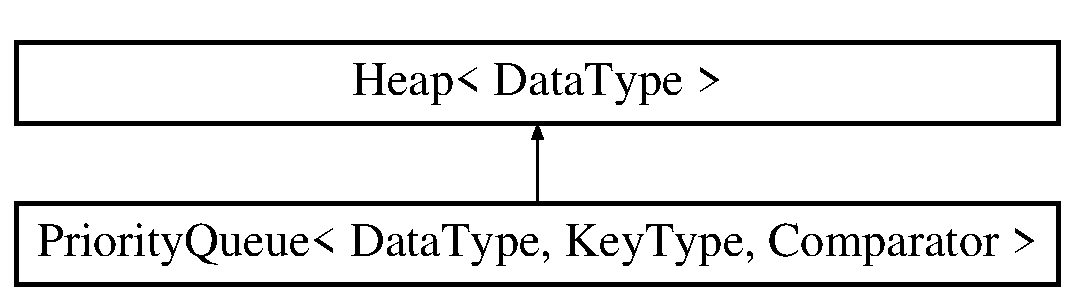
\includegraphics[height=2.000000cm]{class_priority_queue}
\end{center}
\end{figure}
\subsection*{\-Public \-Member \-Functions}
\begin{DoxyCompactItemize}
\item 
\hyperlink{class_priority_queue_a47de2a46cff1d6a6ed30a99c94dc1b14}{\-Priority\-Queue} (int max\-Number=\hyperlink{_priority_queue_8h_a88703212007be018800be64f2f5fde2f}{def\-Max\-Queue\-Size})
\item 
void \hyperlink{class_priority_queue_a61f3339cf0e87c67ed004f8eff0a1bfa}{enqueue} (const \-Data\-Type \&new\-Data\-Item)
\item 
\-Data\-Type \hyperlink{class_priority_queue_a5bc758e313d6244e672ea6e81d695a46}{dequeue} ()
\end{DoxyCompactItemize}
\subsubsection*{template$<$typename Data\-Type, typename Key\-Type = int, typename Comparator = \-Less$<$\-Key\-Type$>$$>$ class Priority\-Queue$<$ Data\-Type, Key\-Type, Comparator $>$}



\subsection{\-Constructor \& \-Destructor \-Documentation}
\hypertarget{class_priority_queue_a47de2a46cff1d6a6ed30a99c94dc1b14}{\index{\-Priority\-Queue@{\-Priority\-Queue}!\-Priority\-Queue@{\-Priority\-Queue}}
\index{\-Priority\-Queue@{\-Priority\-Queue}!PriorityQueue@{\-Priority\-Queue}}
\subsubsection[{\-Priority\-Queue}]{\setlength{\rightskip}{0pt plus 5cm}template$<$typename Data\-Type , typename Key\-Type , typename Comparator $>$ {\bf \-Priority\-Queue}$<$ \-Data\-Type, \-Key\-Type, \-Comparator $>$\-::{\bf \-Priority\-Queue} (
\begin{DoxyParamCaption}
\item[{int}]{max\-Number = {\ttfamily {\bf def\-Max\-Queue\-Size}}}
\end{DoxyParamCaption}
)}}\label{class_priority_queue_a47de2a46cff1d6a6ed30a99c94dc1b14}
\hyperlink{class_priority_queue}{\-Priority\-Queue} \-Constructor

\-This constructor inherently calls the heap consructor


\begin{DoxyParams}{\-Parameters}
{\em max\-Number} & -\/ an integer that sets the max\-Size of the number of data\-Items in the heap array\\
\hline
\end{DoxyParams}
\begin{DoxyReturn}{\-Returns}
none
\end{DoxyReturn}
\begin{DoxyPrecond}{\-Precondition}
there will not be an initialized heap or priority queue 
\end{DoxyPrecond}
\begin{DoxyPostcond}{\-Postcondition}
there will be an initialized heap with the max\-Size, and size set (and priority queue) 
\end{DoxyPostcond}


\subsection{\-Member \-Function \-Documentation}
\hypertarget{class_priority_queue_a5bc758e313d6244e672ea6e81d695a46}{\index{\-Priority\-Queue@{\-Priority\-Queue}!dequeue@{dequeue}}
\index{dequeue@{dequeue}!PriorityQueue@{\-Priority\-Queue}}
\subsubsection[{dequeue}]{\setlength{\rightskip}{0pt plus 5cm}template$<$typename Data\-Type , typename Key\-Type , typename Comparator $>$ \-Data\-Type {\bf \-Priority\-Queue}$<$ \-Data\-Type, \-Key\-Type, \-Comparator $>$\-::{\bf dequeue} (
\begin{DoxyParamCaption}
{}
\end{DoxyParamCaption}
)}}\label{class_priority_queue_a5bc758e313d6244e672ea6e81d695a46}
dequeue function

\-This function calls the remove function of the heap


\begin{DoxyParams}{\-Parameters}
{\em none} & \\
\hline
\end{DoxyParams}
\begin{DoxyReturn}{\-Returns}
\-Data\-Type -\/ the data\-Item that was removed from the priority queue
\end{DoxyReturn}
\begin{DoxyPrecond}{\-Precondition}
the data\-Item of highest priority will be in the priority queue 
\end{DoxyPrecond}
\begin{DoxyPostcond}{\-Postcondition}
the data\-Item of highest priority will not be in the priority queue 
\end{DoxyPostcond}
\hypertarget{class_priority_queue_a61f3339cf0e87c67ed004f8eff0a1bfa}{\index{\-Priority\-Queue@{\-Priority\-Queue}!enqueue@{enqueue}}
\index{enqueue@{enqueue}!PriorityQueue@{\-Priority\-Queue}}
\subsubsection[{enqueue}]{\setlength{\rightskip}{0pt plus 5cm}template$<$typename Data\-Type , typename Key\-Type , typename Comparator $>$ void {\bf \-Priority\-Queue}$<$ \-Data\-Type, \-Key\-Type, \-Comparator $>$\-::{\bf enqueue} (
\begin{DoxyParamCaption}
\item[{const \-Data\-Type \&}]{new\-Data\-Item}
\end{DoxyParamCaption}
)}}\label{class_priority_queue_a61f3339cf0e87c67ed004f8eff0a1bfa}
enqueue function

\-This function calls the insert function of the heap.


\begin{DoxyParams}{\-Parameters}
{\em new\-Data\-Item} & -\/ the data\-Item that is to be placed into the priority queue\\
\hline
\end{DoxyParams}
\begin{DoxyReturn}{\-Returns}
none
\end{DoxyReturn}
\begin{DoxyPrecond}{\-Precondition}
the new\-Data\-Item will not be in the current priority queue 
\end{DoxyPrecond}
\begin{DoxyPostcond}{\-Postcondition}
the data\-Item will be placed into the priority queue if the heap array is not full 
\end{DoxyPostcond}


\-The documentation for this class was generated from the following files\-:\begin{DoxyCompactItemize}
\item 
\hyperlink{_priority_queue_8h}{\-Priority\-Queue.\-h}\item 
\hyperlink{_priority_queue_8cpp}{\-Priority\-Queue.\-cpp}\end{DoxyCompactItemize}

\hypertarget{struct_task_data}{\section{\-Task\-Data \-Struct \-Reference}
\label{struct_task_data}\index{\-Task\-Data@{\-Task\-Data}}
}
\subsection*{\-Public \-Member \-Functions}
\begin{DoxyCompactItemize}
\item 
int \hyperlink{struct_task_data_a58cbe6eec8a86be7b827561a2f4b49c1}{get\-Priority} () const 
\item 
int \hyperlink{struct_task_data_a58cbe6eec8a86be7b827561a2f4b49c1}{get\-Priority} () const 
\end{DoxyCompactItemize}
\subsection*{\-Public \-Attributes}
\begin{DoxyCompactItemize}
\item 
int \hyperlink{struct_task_data_a9d8b606897eb428a62d816b71312e1b7}{priority}
\item 
int \hyperlink{struct_task_data_a126fafee3369b6a2d8734f4e46c670bc}{arrived}
\end{DoxyCompactItemize}


\subsection{\-Member \-Function \-Documentation}
\hypertarget{struct_task_data_a58cbe6eec8a86be7b827561a2f4b49c1}{\index{\-Task\-Data@{\-Task\-Data}!get\-Priority@{get\-Priority}}
\index{get\-Priority@{get\-Priority}!TaskData@{\-Task\-Data}}
\subsubsection[{get\-Priority}]{\setlength{\rightskip}{0pt plus 5cm}int {\bf \-Task\-Data\-::get\-Priority} (
\begin{DoxyParamCaption}
{}
\end{DoxyParamCaption}
) const\hspace{0.3cm}{\ttfamily  \mbox{[}inline\mbox{]}}}}\label{struct_task_data_a58cbe6eec8a86be7b827561a2f4b49c1}
\hypertarget{struct_task_data_a58cbe6eec8a86be7b827561a2f4b49c1}{\index{\-Task\-Data@{\-Task\-Data}!get\-Priority@{get\-Priority}}
\index{get\-Priority@{get\-Priority}!TaskData@{\-Task\-Data}}
\subsubsection[{get\-Priority}]{\setlength{\rightskip}{0pt plus 5cm}int {\bf \-Task\-Data\-::get\-Priority} (
\begin{DoxyParamCaption}
{}
\end{DoxyParamCaption}
) const\hspace{0.3cm}{\ttfamily  \mbox{[}inline\mbox{]}}}}\label{struct_task_data_a58cbe6eec8a86be7b827561a2f4b49c1}


\subsection{\-Member \-Data \-Documentation}
\hypertarget{struct_task_data_a126fafee3369b6a2d8734f4e46c670bc}{\index{\-Task\-Data@{\-Task\-Data}!arrived@{arrived}}
\index{arrived@{arrived}!TaskData@{\-Task\-Data}}
\subsubsection[{arrived}]{\setlength{\rightskip}{0pt plus 5cm}int {\bf \-Task\-Data\-::arrived}}}\label{struct_task_data_a126fafee3369b6a2d8734f4e46c670bc}
\hypertarget{struct_task_data_a9d8b606897eb428a62d816b71312e1b7}{\index{\-Task\-Data@{\-Task\-Data}!priority@{priority}}
\index{priority@{priority}!TaskData@{\-Task\-Data}}
\subsubsection[{priority}]{\setlength{\rightskip}{0pt plus 5cm}int {\bf \-Task\-Data\-::priority}}}\label{struct_task_data_a9d8b606897eb428a62d816b71312e1b7}


\-The documentation for this struct was generated from the following files\-:\begin{DoxyCompactItemize}
\item 
\hyperlink{ossim_8cpp}{ossim.\-cpp}\item 
\hyperlink{ossim_8cs}{ossim.\-cs}\end{DoxyCompactItemize}

\hypertarget{class_test_data}{\section{\-Test\-Data \-Class \-Reference}
\label{class_test_data}\index{\-Test\-Data@{\-Test\-Data}}
}
\subsection*{\-Public \-Member \-Functions}
\begin{DoxyCompactItemize}
\item 
\hyperlink{class_test_data_aa4a3dd519ba3a3ae02956b627d42d123}{\-Test\-Data} ()
\item 
\hyperlink{class_test_data_af4ed2af760afe9e61fcf5333b008b2b9}{$\sim$\-Test\-Data} ()
\item 
void \hyperlink{class_test_data_a72cb0d5febcf77e8a6dd494fa6dff411}{set\-Key} (const string \&new\-Key)
\item 
string \hyperlink{class_test_data_ae20d0a4c5fba891d728c68ac4ec79654}{get\-Key} () const 
\item 
int \hyperlink{class_test_data_af33e667b6962f8a351f7a660a1a24c5e}{get\-Value} () const 
\item 
void \hyperlink{class_test_data_a609b8a4b0e3221bfb0b8cbd9efb108a7}{set\-Key} (int new\-Key)
\item 
int \hyperlink{class_test_data_a85ac27a4361a78d576dd8c10b1f97961}{get\-Key} () const 
\end{DoxyCompactItemize}
\subsection*{\-Static \-Public \-Member \-Functions}
\begin{DoxyCompactItemize}
\item 
static unsigned int \hyperlink{class_test_data_a55f0e2851aa330be9921303107982f98}{hash} (const string \&str)
\end{DoxyCompactItemize}
\subsection*{\-Private \-Attributes}
\begin{DoxyCompactItemize}
\item 
string \hyperlink{class_test_data_a16fe3a9a89c54e55fc56ae88590ae0c8}{key}
\item 
int \hyperlink{class_test_data_a8291f6b900b25a926deb1b2a393dc0ff}{value}
\item 
int \hyperlink{class_test_data_adafb60a315eaa088791c9e40f4a2618f}{key\-Field}
\end{DoxyCompactItemize}
\subsection*{\-Static \-Private \-Attributes}
\begin{DoxyCompactItemize}
\item 
static int \hyperlink{class_test_data_a9209c5345dda5dcb483b9c972fafc495}{count} = 0
\end{DoxyCompactItemize}


\subsection{\-Constructor \& \-Destructor \-Documentation}
\hypertarget{class_test_data_aa4a3dd519ba3a3ae02956b627d42d123}{\index{\-Test\-Data@{\-Test\-Data}!\-Test\-Data@{\-Test\-Data}}
\index{\-Test\-Data@{\-Test\-Data}!TestData@{\-Test\-Data}}
\subsubsection[{\-Test\-Data}]{\setlength{\rightskip}{0pt plus 5cm}{\bf \-Test\-Data\-::\-Test\-Data} (
\begin{DoxyParamCaption}
{}
\end{DoxyParamCaption}
)}}\label{class_test_data_aa4a3dd519ba3a3ae02956b627d42d123}
\hypertarget{class_test_data_af4ed2af760afe9e61fcf5333b008b2b9}{\index{\-Test\-Data@{\-Test\-Data}!$\sim$\-Test\-Data@{$\sim$\-Test\-Data}}
\index{$\sim$\-Test\-Data@{$\sim$\-Test\-Data}!TestData@{\-Test\-Data}}
\subsubsection[{$\sim$\-Test\-Data}]{\setlength{\rightskip}{0pt plus 5cm}{\bf \-Test\-Data\-::$\sim$\-Test\-Data} (
\begin{DoxyParamCaption}
{}
\end{DoxyParamCaption}
)}}\label{class_test_data_af4ed2af760afe9e61fcf5333b008b2b9}


\subsection{\-Member \-Function \-Documentation}
\hypertarget{class_test_data_ae20d0a4c5fba891d728c68ac4ec79654}{\index{\-Test\-Data@{\-Test\-Data}!get\-Key@{get\-Key}}
\index{get\-Key@{get\-Key}!TestData@{\-Test\-Data}}
\subsubsection[{get\-Key}]{\setlength{\rightskip}{0pt plus 5cm}string {\bf \-Test\-Data\-::get\-Key} (
\begin{DoxyParamCaption}
{}
\end{DoxyParamCaption}
) const}}\label{class_test_data_ae20d0a4c5fba891d728c68ac4ec79654}
\hypertarget{class_test_data_a85ac27a4361a78d576dd8c10b1f97961}{\index{\-Test\-Data@{\-Test\-Data}!get\-Key@{get\-Key}}
\index{get\-Key@{get\-Key}!TestData@{\-Test\-Data}}
\subsubsection[{get\-Key}]{\setlength{\rightskip}{0pt plus 5cm}int {\bf \-Test\-Data\-::get\-Key} (
\begin{DoxyParamCaption}
{}
\end{DoxyParamCaption}
) const\hspace{0.3cm}{\ttfamily  \mbox{[}inline\mbox{]}}}}\label{class_test_data_a85ac27a4361a78d576dd8c10b1f97961}
\hypertarget{class_test_data_af33e667b6962f8a351f7a660a1a24c5e}{\index{\-Test\-Data@{\-Test\-Data}!get\-Value@{get\-Value}}
\index{get\-Value@{get\-Value}!TestData@{\-Test\-Data}}
\subsubsection[{get\-Value}]{\setlength{\rightskip}{0pt plus 5cm}int {\bf \-Test\-Data\-::get\-Value} (
\begin{DoxyParamCaption}
{}
\end{DoxyParamCaption}
) const}}\label{class_test_data_af33e667b6962f8a351f7a660a1a24c5e}
\hypertarget{class_test_data_a55f0e2851aa330be9921303107982f98}{\index{\-Test\-Data@{\-Test\-Data}!hash@{hash}}
\index{hash@{hash}!TestData@{\-Test\-Data}}
\subsubsection[{hash}]{\setlength{\rightskip}{0pt plus 5cm}unsigned int {\bf \-Test\-Data\-::hash} (
\begin{DoxyParamCaption}
\item[{const string \&}]{str}
\end{DoxyParamCaption}
)\hspace{0.3cm}{\ttfamily  \mbox{[}static\mbox{]}}}}\label{class_test_data_a55f0e2851aa330be9921303107982f98}
\hypertarget{class_test_data_a72cb0d5febcf77e8a6dd494fa6dff411}{\index{\-Test\-Data@{\-Test\-Data}!set\-Key@{set\-Key}}
\index{set\-Key@{set\-Key}!TestData@{\-Test\-Data}}
\subsubsection[{set\-Key}]{\setlength{\rightskip}{0pt plus 5cm}void {\bf \-Test\-Data\-::set\-Key} (
\begin{DoxyParamCaption}
\item[{const string \&}]{new\-Key}
\end{DoxyParamCaption}
)}}\label{class_test_data_a72cb0d5febcf77e8a6dd494fa6dff411}
\hypertarget{class_test_data_a609b8a4b0e3221bfb0b8cbd9efb108a7}{\index{\-Test\-Data@{\-Test\-Data}!set\-Key@{set\-Key}}
\index{set\-Key@{set\-Key}!TestData@{\-Test\-Data}}
\subsubsection[{set\-Key}]{\setlength{\rightskip}{0pt plus 5cm}void {\bf \-Test\-Data\-::set\-Key} (
\begin{DoxyParamCaption}
\item[{int}]{new\-Key}
\end{DoxyParamCaption}
)\hspace{0.3cm}{\ttfamily  \mbox{[}inline\mbox{]}}}}\label{class_test_data_a609b8a4b0e3221bfb0b8cbd9efb108a7}


\subsection{\-Member \-Data \-Documentation}
\hypertarget{class_test_data_a9209c5345dda5dcb483b9c972fafc495}{\index{\-Test\-Data@{\-Test\-Data}!count@{count}}
\index{count@{count}!TestData@{\-Test\-Data}}
\subsubsection[{count}]{\setlength{\rightskip}{0pt plus 5cm}int {\bf \-Test\-Data\-::count} = 0\hspace{0.3cm}{\ttfamily  \mbox{[}static, private\mbox{]}}}}\label{class_test_data_a9209c5345dda5dcb483b9c972fafc495}
\hypertarget{class_test_data_a16fe3a9a89c54e55fc56ae88590ae0c8}{\index{\-Test\-Data@{\-Test\-Data}!key@{key}}
\index{key@{key}!TestData@{\-Test\-Data}}
\subsubsection[{key}]{\setlength{\rightskip}{0pt plus 5cm}string {\bf \-Test\-Data\-::key}\hspace{0.3cm}{\ttfamily  \mbox{[}private\mbox{]}}}}\label{class_test_data_a16fe3a9a89c54e55fc56ae88590ae0c8}
\hypertarget{class_test_data_adafb60a315eaa088791c9e40f4a2618f}{\index{\-Test\-Data@{\-Test\-Data}!key\-Field@{key\-Field}}
\index{key\-Field@{key\-Field}!TestData@{\-Test\-Data}}
\subsubsection[{key\-Field}]{\setlength{\rightskip}{0pt plus 5cm}int {\bf \-Test\-Data\-::key\-Field}\hspace{0.3cm}{\ttfamily  \mbox{[}private\mbox{]}}}}\label{class_test_data_adafb60a315eaa088791c9e40f4a2618f}
\hypertarget{class_test_data_a8291f6b900b25a926deb1b2a393dc0ff}{\index{\-Test\-Data@{\-Test\-Data}!value@{value}}
\index{value@{value}!TestData@{\-Test\-Data}}
\subsubsection[{value}]{\setlength{\rightskip}{0pt plus 5cm}int {\bf \-Test\-Data\-::value}\hspace{0.3cm}{\ttfamily  \mbox{[}private\mbox{]}}}}\label{class_test_data_a8291f6b900b25a926deb1b2a393dc0ff}


\-The documentation for this class was generated from the following files\-:\begin{DoxyCompactItemize}
\item 
\hyperlink{test10_8cpp}{test10.\-cpp}\item 
\hyperlink{test9_8cpp}{test9.\-cpp}\end{DoxyCompactItemize}

\hypertarget{class_test_data_item}{\section{\-Test\-Data\-Item$<$ \-Key\-Type $>$ \-Class \-Template \-Reference}
\label{class_test_data_item}\index{\-Test\-Data\-Item$<$ Key\-Type $>$@{\-Test\-Data\-Item$<$ Key\-Type $>$}}
}
\subsection*{\-Public \-Member \-Functions}
\begin{DoxyCompactItemize}
\item 
\hyperlink{class_test_data_item_adfbd4f5d142caf3d95c96940f96c1d85}{\-Test\-Data\-Item} ()
\item 
void \hyperlink{class_test_data_item_a84667429c081b1dbb212956c88011216}{set\-Priority} (\-Key\-Type new\-Pty)
\item 
\-Key\-Type \hyperlink{class_test_data_item_ac1632213d959555ec8f5aee8a1505d72}{get\-Priority} () const 
\end{DoxyCompactItemize}
\subsection*{\-Private \-Attributes}
\begin{DoxyCompactItemize}
\item 
\-Key\-Type \hyperlink{class_test_data_item_a9b1a2617cb7a831206d189559e8e2e8b}{priority}
\end{DoxyCompactItemize}
\subsubsection*{template$<$typename Key\-Type$>$ class Test\-Data\-Item$<$ Key\-Type $>$}



\subsection{\-Constructor \& \-Destructor \-Documentation}
\hypertarget{class_test_data_item_adfbd4f5d142caf3d95c96940f96c1d85}{\index{\-Test\-Data\-Item@{\-Test\-Data\-Item}!\-Test\-Data\-Item@{\-Test\-Data\-Item}}
\index{\-Test\-Data\-Item@{\-Test\-Data\-Item}!TestDataItem@{\-Test\-Data\-Item}}
\subsubsection[{\-Test\-Data\-Item}]{\setlength{\rightskip}{0pt plus 5cm}template$<$typename Key\-Type $>$ {\bf \-Test\-Data\-Item}$<$ \-Key\-Type $>$\-::{\bf \-Test\-Data\-Item} (
\begin{DoxyParamCaption}
{}
\end{DoxyParamCaption}
)\hspace{0.3cm}{\ttfamily  \mbox{[}inline\mbox{]}}}}\label{class_test_data_item_adfbd4f5d142caf3d95c96940f96c1d85}


\subsection{\-Member \-Function \-Documentation}
\hypertarget{class_test_data_item_ac1632213d959555ec8f5aee8a1505d72}{\index{\-Test\-Data\-Item@{\-Test\-Data\-Item}!get\-Priority@{get\-Priority}}
\index{get\-Priority@{get\-Priority}!TestDataItem@{\-Test\-Data\-Item}}
\subsubsection[{get\-Priority}]{\setlength{\rightskip}{0pt plus 5cm}template$<$typename Key\-Type $>$ \-Key\-Type {\bf \-Test\-Data\-Item}$<$ \-Key\-Type $>$\-::{\bf get\-Priority} (
\begin{DoxyParamCaption}
{}
\end{DoxyParamCaption}
) const\hspace{0.3cm}{\ttfamily  \mbox{[}inline\mbox{]}}}}\label{class_test_data_item_ac1632213d959555ec8f5aee8a1505d72}
\hypertarget{class_test_data_item_a84667429c081b1dbb212956c88011216}{\index{\-Test\-Data\-Item@{\-Test\-Data\-Item}!set\-Priority@{set\-Priority}}
\index{set\-Priority@{set\-Priority}!TestDataItem@{\-Test\-Data\-Item}}
\subsubsection[{set\-Priority}]{\setlength{\rightskip}{0pt plus 5cm}template$<$typename Key\-Type $>$ void {\bf \-Test\-Data\-Item}$<$ \-Key\-Type $>$\-::{\bf set\-Priority} (
\begin{DoxyParamCaption}
\item[{\-Key\-Type}]{new\-Pty}
\end{DoxyParamCaption}
)\hspace{0.3cm}{\ttfamily  \mbox{[}inline\mbox{]}}}}\label{class_test_data_item_a84667429c081b1dbb212956c88011216}


\subsection{\-Member \-Data \-Documentation}
\hypertarget{class_test_data_item_a9b1a2617cb7a831206d189559e8e2e8b}{\index{\-Test\-Data\-Item@{\-Test\-Data\-Item}!priority@{priority}}
\index{priority@{priority}!TestDataItem@{\-Test\-Data\-Item}}
\subsubsection[{priority}]{\setlength{\rightskip}{0pt plus 5cm}template$<$typename Key\-Type $>$ \-Key\-Type {\bf \-Test\-Data\-Item}$<$ \-Key\-Type $>$\-::{\bf priority}\hspace{0.3cm}{\ttfamily  \mbox{[}private\mbox{]}}}}\label{class_test_data_item_a9b1a2617cb7a831206d189559e8e2e8b}


\-The documentation for this class was generated from the following file\-:\begin{DoxyCompactItemize}
\item 
\hyperlink{test11_8cpp}{test11.\-cpp}\end{DoxyCompactItemize}

\chapter{\-File \-Documentation}
\hypertarget{config_8h}{\section{config.\-h \-File \-Reference}
\label{config_8h}\index{config.\-h@{config.\-h}}
}
\subsection*{\-Defines}
\begin{DoxyCompactItemize}
\item 
\#define \hyperlink{config_8h_a37256be1bc236d447e0bfb4668d06e08}{\-L\-A\-B12\-\_\-\-T\-E\-S\-T1}~1
\begin{DoxyCompactList}\small\item\em set all config testing to one to enable all programming exercises \end{DoxyCompactList}\item 
\#define \hyperlink{config_8h_a4e475097daefad258dd91becac6afa97}{\-L\-A\-B12\-\_\-\-T\-E\-S\-T2}~1
\item 
\#define \hyperlink{config_8h_a0796ef74cc24d4f0e3eeb82b48dc8d3e}{\-L\-A\-B12\-\_\-\-T\-E\-S\-T3}~1
\end{DoxyCompactItemize}


\subsection{\-Define \-Documentation}
\hypertarget{config_8h_a37256be1bc236d447e0bfb4668d06e08}{\index{config.\-h@{config.\-h}!\-L\-A\-B12\-\_\-\-T\-E\-S\-T1@{\-L\-A\-B12\-\_\-\-T\-E\-S\-T1}}
\index{\-L\-A\-B12\-\_\-\-T\-E\-S\-T1@{\-L\-A\-B12\-\_\-\-T\-E\-S\-T1}!config.h@{config.\-h}}
\subsubsection[{\-L\-A\-B12\-\_\-\-T\-E\-S\-T1}]{\setlength{\rightskip}{0pt plus 5cm}\#define {\bf \-L\-A\-B12\-\_\-\-T\-E\-S\-T1}~1}}\label{config_8h_a37256be1bc236d447e0bfb4668d06e08}


set all config testing to one to enable all programming exercises 

\hyperlink{class_weighted_graph}{\-Weighted\-Graph} class configuration file. \-Activate test \#\-N by defining the corresponding \-L\-A\-B12\-\_\-\-T\-E\-S\-T\-N to have the value 1. \hypertarget{config_8h_a4e475097daefad258dd91becac6afa97}{\index{config.\-h@{config.\-h}!\-L\-A\-B12\-\_\-\-T\-E\-S\-T2@{\-L\-A\-B12\-\_\-\-T\-E\-S\-T2}}
\index{\-L\-A\-B12\-\_\-\-T\-E\-S\-T2@{\-L\-A\-B12\-\_\-\-T\-E\-S\-T2}!config.h@{config.\-h}}
\subsubsection[{\-L\-A\-B12\-\_\-\-T\-E\-S\-T2}]{\setlength{\rightskip}{0pt plus 5cm}\#define {\bf \-L\-A\-B12\-\_\-\-T\-E\-S\-T2}~1}}\label{config_8h_a4e475097daefad258dd91becac6afa97}
\hypertarget{config_8h_a0796ef74cc24d4f0e3eeb82b48dc8d3e}{\index{config.\-h@{config.\-h}!\-L\-A\-B12\-\_\-\-T\-E\-S\-T3@{\-L\-A\-B12\-\_\-\-T\-E\-S\-T3}}
\index{\-L\-A\-B12\-\_\-\-T\-E\-S\-T3@{\-L\-A\-B12\-\_\-\-T\-E\-S\-T3}!config.h@{config.\-h}}
\subsubsection[{\-L\-A\-B12\-\_\-\-T\-E\-S\-T3}]{\setlength{\rightskip}{0pt plus 5cm}\#define {\bf \-L\-A\-B12\-\_\-\-T\-E\-S\-T3}~1}}\label{config_8h_a0796ef74cc24d4f0e3eeb82b48dc8d3e}

\hypertarget{_heap_8cpp}{\section{\-Heap.\-cpp \-File \-Reference}
\label{_heap_8cpp}\index{\-Heap.\-cpp@{\-Heap.\-cpp}}
}


\-This program contains the basic function for manipulating data in the heap.  


{\ttfamily \#include \char`\"{}\-Heap.\-h\char`\"{}}\*


\subsection{\-Detailed \-Description}
\-This program contains the basic function for manipulating data in the heap. \begin{DoxyAuthor}{\-Author}
\-Henry \-Huffman 
\end{DoxyAuthor}
\begin{DoxyVersion}{\-Version}
1.\-1
\end{DoxyVersion}
\-More specifically, this program has the following basic member functions\-: heap constructor, copy constructor, overloaded = operator, and heap deconstructor. \-This program also contains the following functions\-: insert, remove, clear, is\-Empty, is\-Full, show\-Structure, and write\-Levels. \-There are also several helper functions which are also used to help in manipulating data. \-These functions being\-: show\-Subtree, get\-Left, get\-Right, get\-Parent, heap up, and heap down.

\begin{DoxyDate}{\-Date}
\-Friday, \-October 17th, 2014 
\end{DoxyDate}

\hypertarget{_heap_8h}{\section{\-Heap.\-h \-File \-Reference}
\label{_heap_8h}\index{\-Heap.\-h@{\-Heap.\-h}}
}
{\ttfamily \#include $<$stdexcept$>$}\*
{\ttfamily \#include $<$iostream$>$}\*
{\ttfamily \#include $<$cstdlib$>$}\*
\subsection*{\-Classes}
\begin{DoxyCompactItemize}
\item 
class \hyperlink{class_less}{\-Less$<$ Key\-Type $>$}
\item 
class \hyperlink{class_heap}{\-Heap$<$ Data\-Type, Key\-Type, Comparator $>$}
\end{DoxyCompactItemize}

\hypertarget{heapsort_8cs}{\section{heapsort.\-cs \-File \-Reference}
\label{heapsort_8cs}\index{heapsort.\-cs@{heapsort.\-cs}}
}
\subsection*{\-Functions}
\begin{DoxyCompactItemize}
\item 
{\footnotesize template$<$typename Data\-Type $>$ }\\void \hyperlink{heapsort_8cs_ace0c151b0a221e24a1aad0bf9a821c2f}{move\-Down} (\-Data\-Type data\-Items\mbox{[}$\,$\mbox{]}, int root, int size)
\item 
{\footnotesize template$<$typename Data\-Type $>$ }\\void \hyperlink{heapsort_8cs_a1b9d07732ab0ab5fb1c3fabfb8ba4f4b}{heap\-Sort} (\-Data\-Type data\-Items\mbox{[}$\,$\mbox{]}, int size)
\end{DoxyCompactItemize}


\subsection{\-Function \-Documentation}
\hypertarget{heapsort_8cs_a1b9d07732ab0ab5fb1c3fabfb8ba4f4b}{\index{heapsort.\-cs@{heapsort.\-cs}!heap\-Sort@{heap\-Sort}}
\index{heap\-Sort@{heap\-Sort}!heapsort.cs@{heapsort.\-cs}}
\subsubsection[{heap\-Sort}]{\setlength{\rightskip}{0pt plus 5cm}template$<$typename Data\-Type $>$ void {\bf heap\-Sort} (
\begin{DoxyParamCaption}
\item[{\-Data\-Type}]{data\-Items\mbox{[}$\,$\mbox{]}, }
\item[{int}]{size}
\end{DoxyParamCaption}
)}}\label{heapsort_8cs_a1b9d07732ab0ab5fb1c3fabfb8ba4f4b}
\hypertarget{heapsort_8cs_ace0c151b0a221e24a1aad0bf9a821c2f}{\index{heapsort.\-cs@{heapsort.\-cs}!move\-Down@{move\-Down}}
\index{move\-Down@{move\-Down}!heapsort.cs@{heapsort.\-cs}}
\subsubsection[{move\-Down}]{\setlength{\rightskip}{0pt plus 5cm}template$<$typename Data\-Type $>$ void {\bf move\-Down} (
\begin{DoxyParamCaption}
\item[{\-Data\-Type}]{data\-Items\mbox{[}$\,$\mbox{]}, }
\item[{int}]{root, }
\item[{int}]{size}
\end{DoxyParamCaption}
)}}\label{heapsort_8cs_ace0c151b0a221e24a1aad0bf9a821c2f}

\hypertarget{ossim_8cpp}{\section{ossim.\-cpp \-File \-Reference}
\label{ossim_8cpp}\index{ossim.\-cpp@{ossim.\-cpp}}
}


\-This program uses a priority queue to simulate a line.  


{\ttfamily \#include $<$iostream$>$}\*
{\ttfamily \#include $<$cstdlib$>$}\*
{\ttfamily \#include \char`\"{}\-Priority\-Queue.\-cpp\char`\"{}}\*
\subsection*{\-Classes}
\begin{DoxyCompactItemize}
\item 
struct \hyperlink{struct_task_data}{\-Task\-Data}
\end{DoxyCompactItemize}
\subsection*{\-Functions}
\begin{DoxyCompactItemize}
\item 
int \hyperlink{ossim_8cpp_ae66f6b31b5ad750f1fe042a706a4e3d4}{main} ()
\end{DoxyCompactItemize}


\subsection{\-Detailed \-Description}
\-This program uses a priority queue to simulate a line. \begin{DoxyAuthor}{\-Author}
\-Henry \-Huffman 
\end{DoxyAuthor}
\begin{DoxyVersion}{\-Version}
1.\-1
\end{DoxyVersion}
\-Moreover, this program will generate random numbers for a specified amount of times. \-Then it will dequeue one data item per minute and enqueue randomly generated values. \-The value of the dequeued data\-Item will be output.

\begin{DoxyDate}{\-Date}
\-Tuesday, \-October 28th, 2014 
\end{DoxyDate}


\subsection{\-Function \-Documentation}
\hypertarget{ossim_8cpp_ae66f6b31b5ad750f1fe042a706a4e3d4}{\index{ossim.\-cpp@{ossim.\-cpp}!main@{main}}
\index{main@{main}!ossim.cpp@{ossim.\-cpp}}
\subsubsection[{main}]{\setlength{\rightskip}{0pt plus 5cm}int {\bf main} (
\begin{DoxyParamCaption}
{}
\end{DoxyParamCaption}
)}}\label{ossim_8cpp_ae66f6b31b5ad750f1fe042a706a4e3d4}

\hypertarget{ossim_8cs}{\section{ossim.\-cs \-File \-Reference}
\label{ossim_8cs}\index{ossim.\-cs@{ossim.\-cs}}
}
{\ttfamily \#include $<$iostream$>$}\*
{\ttfamily \#include $<$cstdlib$>$}\*
{\ttfamily \#include \char`\"{}\-Priority\-Queue.\-cpp\char`\"{}}\*
\subsection*{\-Classes}
\begin{DoxyCompactItemize}
\item 
struct \hyperlink{struct_task_data}{\-Task\-Data}
\end{DoxyCompactItemize}
\subsection*{\-Functions}
\begin{DoxyCompactItemize}
\item 
int \hyperlink{ossim_8cs_ae66f6b31b5ad750f1fe042a706a4e3d4}{main} ()
\end{DoxyCompactItemize}


\subsection{\-Function \-Documentation}
\hypertarget{ossim_8cs_ae66f6b31b5ad750f1fe042a706a4e3d4}{\index{ossim.\-cs@{ossim.\-cs}!main@{main}}
\index{main@{main}!ossim.cs@{ossim.\-cs}}
\subsubsection[{main}]{\setlength{\rightskip}{0pt plus 5cm}int {\bf main} (
\begin{DoxyParamCaption}
{}
\end{DoxyParamCaption}
)}}\label{ossim_8cs_ae66f6b31b5ad750f1fe042a706a4e3d4}

\hypertarget{_priority_queue_8cpp}{\section{\-Priority\-Queue.\-cpp \-File \-Reference}
\label{_priority_queue_8cpp}\index{\-Priority\-Queue.\-cpp@{\-Priority\-Queue.\-cpp}}
}


\-The priority queue uses the predefined heap functions to perform basic priority queue operations.  


{\ttfamily \#include \char`\"{}\-Priority\-Queue.\-h\char`\"{}}\*


\subsection{\-Detailed \-Description}
\-The priority queue uses the predefined heap functions to perform basic priority queue operations. \begin{DoxyAuthor}{\-Author}
\-Henry \-Huffman 
\end{DoxyAuthor}
\begin{DoxyVersion}{\-Version}
1.\-1
\end{DoxyVersion}
\-More specifically, this program contains the following functions\-: priorirty queue constructor, enqueue, and dequeue. \begin{DoxyDate}{\-Date}
\-Friday, \-October 17th, 2014 
\end{DoxyDate}

\hypertarget{_priority_queue_8h}{\section{\-Priority\-Queue.\-h \-File \-Reference}
\label{_priority_queue_8h}\index{\-Priority\-Queue.\-h@{\-Priority\-Queue.\-h}}
}
{\ttfamily \#include $<$stdexcept$>$}\*
{\ttfamily \#include $<$iostream$>$}\*
{\ttfamily \#include \char`\"{}\-Heap.\-cpp\char`\"{}}\*
\subsection*{\-Classes}
\begin{DoxyCompactItemize}
\item 
class \hyperlink{class_priority_queue}{\-Priority\-Queue$<$ Data\-Type, Key\-Type, Comparator $>$}
\end{DoxyCompactItemize}
\subsection*{\-Variables}
\begin{DoxyCompactItemize}
\item 
const int \hyperlink{_priority_queue_8h_a88703212007be018800be64f2f5fde2f}{def\-Max\-Queue\-Size} = 10
\end{DoxyCompactItemize}


\subsection{\-Variable \-Documentation}
\hypertarget{_priority_queue_8h_a88703212007be018800be64f2f5fde2f}{\index{\-Priority\-Queue.\-h@{\-Priority\-Queue.\-h}!def\-Max\-Queue\-Size@{def\-Max\-Queue\-Size}}
\index{def\-Max\-Queue\-Size@{def\-Max\-Queue\-Size}!PriorityQueue.h@{\-Priority\-Queue.\-h}}
\subsubsection[{def\-Max\-Queue\-Size}]{\setlength{\rightskip}{0pt plus 5cm}const int {\bf def\-Max\-Queue\-Size} = 10}}\label{_priority_queue_8h_a88703212007be018800be64f2f5fde2f}

\hypertarget{show11_8cpp}{\section{show11.\-cpp \-File \-Reference}
\label{show11_8cpp}\index{show11.\-cpp@{show11.\-cpp}}
}

\hypertarget{test11_8cpp}{\section{test11.\-cpp \-File \-Reference}
\label{test11_8cpp}\index{test11.\-cpp@{test11.\-cpp}}
}
{\ttfamily \#include $<$iostream$>$}\*
{\ttfamily \#include $<$string$>$}\*
{\ttfamily \#include $<$cctype$>$}\*
{\ttfamily \#include \char`\"{}\-Heap.\-cpp\char`\"{}}\*
{\ttfamily \#include \char`\"{}config.\-h\char`\"{}}\*
\subsection*{\-Classes}
\begin{DoxyCompactItemize}
\item 
class \hyperlink{class_test_data_item}{\-Test\-Data\-Item$<$ Key\-Type $>$}
\item 
class \hyperlink{class_greater}{\-Greater$<$ Key\-Type $>$}
\end{DoxyCompactItemize}
\subsection*{\-Functions}
\begin{DoxyCompactItemize}
\item 
void \hyperlink{test11_8cpp_a0d20b69b0ad703df78459e1033d5c1d4}{print\-Help} ()
\item 
int \hyperlink{test11_8cpp_ae66f6b31b5ad750f1fe042a706a4e3d4}{main} ()
\end{DoxyCompactItemize}


\subsection{\-Function \-Documentation}
\hypertarget{test11_8cpp_ae66f6b31b5ad750f1fe042a706a4e3d4}{\index{test11.\-cpp@{test11.\-cpp}!main@{main}}
\index{main@{main}!test11.cpp@{test11.\-cpp}}
\subsubsection[{main}]{\setlength{\rightskip}{0pt plus 5cm}int {\bf main} (
\begin{DoxyParamCaption}
{}
\end{DoxyParamCaption}
)}}\label{test11_8cpp_ae66f6b31b5ad750f1fe042a706a4e3d4}
\hypertarget{test11_8cpp_a0d20b69b0ad703df78459e1033d5c1d4}{\index{test11.\-cpp@{test11.\-cpp}!print\-Help@{print\-Help}}
\index{print\-Help@{print\-Help}!test11.cpp@{test11.\-cpp}}
\subsubsection[{print\-Help}]{\setlength{\rightskip}{0pt plus 5cm}void {\bf print\-Help} (
\begin{DoxyParamCaption}
{}
\end{DoxyParamCaption}
)}}\label{test11_8cpp_a0d20b69b0ad703df78459e1033d5c1d4}

\hypertarget{test11hs_8cpp}{\section{test11hs.\-cpp \-File \-Reference}
\label{test11hs_8cpp}\index{test11hs.\-cpp@{test11hs.\-cpp}}
}
{\ttfamily \#include $<$iostream$>$}\*
{\ttfamily \#include \char`\"{}heapsort.\-cpp\char`\"{}}\*
\subsection*{\-Classes}
\begin{DoxyCompactItemize}
\item 
class \hyperlink{class_test_data}{\-Test\-Data}
\end{DoxyCompactItemize}
\subsection*{\-Functions}
\begin{DoxyCompactItemize}
\item 
int \hyperlink{test11hs_8cpp_ae66f6b31b5ad750f1fe042a706a4e3d4}{main} ()
\end{DoxyCompactItemize}
\subsection*{\-Variables}
\begin{DoxyCompactItemize}
\item 
const int \hyperlink{test11hs_8cpp_af9ecea2a656a85cc42eb181a9976ad31}{\-M\-A\-X\-\_\-\-N\-U\-M\-\_\-\-D\-A\-T\-A\-\_\-\-I\-T\-E\-M\-S} = 10
\end{DoxyCompactItemize}


\subsection{\-Function \-Documentation}
\hypertarget{test11hs_8cpp_ae66f6b31b5ad750f1fe042a706a4e3d4}{\index{test11hs.\-cpp@{test11hs.\-cpp}!main@{main}}
\index{main@{main}!test11hs.cpp@{test11hs.\-cpp}}
\subsubsection[{main}]{\setlength{\rightskip}{0pt plus 5cm}int {\bf main} (
\begin{DoxyParamCaption}
{}
\end{DoxyParamCaption}
)}}\label{test11hs_8cpp_ae66f6b31b5ad750f1fe042a706a4e3d4}


\subsection{\-Variable \-Documentation}
\hypertarget{test11hs_8cpp_af9ecea2a656a85cc42eb181a9976ad31}{\index{test11hs.\-cpp@{test11hs.\-cpp}!\-M\-A\-X\-\_\-\-N\-U\-M\-\_\-\-D\-A\-T\-A\-\_\-\-I\-T\-E\-M\-S@{\-M\-A\-X\-\_\-\-N\-U\-M\-\_\-\-D\-A\-T\-A\-\_\-\-I\-T\-E\-M\-S}}
\index{\-M\-A\-X\-\_\-\-N\-U\-M\-\_\-\-D\-A\-T\-A\-\_\-\-I\-T\-E\-M\-S@{\-M\-A\-X\-\_\-\-N\-U\-M\-\_\-\-D\-A\-T\-A\-\_\-\-I\-T\-E\-M\-S}!test11hs.cpp@{test11hs.\-cpp}}
\subsubsection[{\-M\-A\-X\-\_\-\-N\-U\-M\-\_\-\-D\-A\-T\-A\-\_\-\-I\-T\-E\-M\-S}]{\setlength{\rightskip}{0pt plus 5cm}const int {\bf \-M\-A\-X\-\_\-\-N\-U\-M\-\_\-\-D\-A\-T\-A\-\_\-\-I\-T\-E\-M\-S} = 10}}\label{test11hs_8cpp_af9ecea2a656a85cc42eb181a9976ad31}

\hypertarget{test11pq_8cpp}{\section{test11pq.\-cpp \-File \-Reference}
\label{test11pq_8cpp}\index{test11pq.\-cpp@{test11pq.\-cpp}}
}
{\ttfamily \#include $<$iostream$>$}\*
{\ttfamily \#include $<$cctype$>$}\*
{\ttfamily \#include \char`\"{}\-Priority\-Queue.\-cpp\char`\"{}}\*
\subsection*{\-Classes}
\begin{DoxyCompactItemize}
\item 
class \hyperlink{class_test_data}{\-Test\-Data}
\end{DoxyCompactItemize}
\subsection*{\-Functions}
\begin{DoxyCompactItemize}
\item 
void \hyperlink{test11pq_8cpp_a0d20b69b0ad703df78459e1033d5c1d4}{print\-Help} ()
\item 
int \hyperlink{test11pq_8cpp_ae66f6b31b5ad750f1fe042a706a4e3d4}{main} ()
\end{DoxyCompactItemize}


\subsection{\-Function \-Documentation}
\hypertarget{test11pq_8cpp_ae66f6b31b5ad750f1fe042a706a4e3d4}{\index{test11pq.\-cpp@{test11pq.\-cpp}!main@{main}}
\index{main@{main}!test11pq.cpp@{test11pq.\-cpp}}
\subsubsection[{main}]{\setlength{\rightskip}{0pt plus 5cm}int {\bf main} (
\begin{DoxyParamCaption}
{}
\end{DoxyParamCaption}
)}}\label{test11pq_8cpp_ae66f6b31b5ad750f1fe042a706a4e3d4}
\hypertarget{test11pq_8cpp_a0d20b69b0ad703df78459e1033d5c1d4}{\index{test11pq.\-cpp@{test11pq.\-cpp}!print\-Help@{print\-Help}}
\index{print\-Help@{print\-Help}!test11pq.cpp@{test11pq.\-cpp}}
\subsubsection[{print\-Help}]{\setlength{\rightskip}{0pt plus 5cm}void {\bf print\-Help} (
\begin{DoxyParamCaption}
{}
\end{DoxyParamCaption}
)}}\label{test11pq_8cpp_a0d20b69b0ad703df78459e1033d5c1d4}

\printindex
\end{document}
